\chapter{Aplicación del método}
\label{Metodo}
El desarrollo de la metodología propuesta en el proyecto es el capítulo central de este documento, aquí se presenta el diseño y la implementación de los algoritmos desarrollados en el proyecto.


%En seguida, se inicia con la presentación de trabajos que dejan ver la importancia que este tipo de propuestas tiene para la comunidad científica internacional.


%\section{DISEÑO DEL PROTOTIPO} 
%Aquí se describe cada uno de los componentes del diseño que compone esta investigación.

\section{Diseño del grafo}
\textit{Inspirados en el grafo del caso de estudio descrito en la sección \ref{Sec:CMMN}, se observó que en la notación de modelado CMMN (ver figura \ref{EjCMMN}) se cuenta con un conjunto de tareas o actividades y de flujos entre ellas, que pueden ser opcionales. Se vio cómo esta situación podía modelarse en un grafo, en el que el problema a solucionar consiste en qué tareas realizar de \textbf{L} etapas consecutivas, para alcanzar al final el objetivo.}

\textit{Un grafo dirigido y conexo permite modelar la estructura de procesos de decisión por etapas de estado y tiempo finitos, como el quw se aprecia en la figura \ref{GrafoEtapas}, cuyos nodos, entre cada dos etapas, tienen las características de un grafo bipartito, es decir que, entre acciones de la misma etapa no deben existir aristas; además, como es conexo, se garantiza que exista al menos una arista que conecte dos etapas sucesivas, así, cada nodo, (excepto los de la última etapa), debe estar conectado al menos con un nodo de la etapa siguiente.}

\begin{figure}[H]
  \centering
    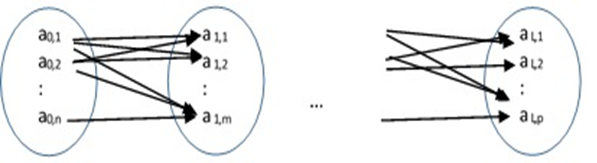
\includegraphics[scale=0.8]{GrafoEtapas.png}
  \caption{Grafo por etapas}
  \label{GrafoEtapas}
\end{figure}

\textit{El grafo es un <<grafo por etapas>>, característica definida en la sección \ref{ConcepGraph}, y el problema que se quiera solucionar debe modelarse como este grafo, con número fijo $L$ de etapas, para que sea susceptible de emplear la aplicación propuesta en esta tesis, por medio de la cual ha de encontrar un camino recomendable para alcanzar un objetivo dado.}

\section{Diseño del modelo matemático}
\label{mat}
Ya se ha dicho que cada uno de los nodos del grafo se constituye en un \textit{ bandit}, pero se desconoce el valor de utilidad que se obtendrá al pasar por cada uno de ellos y solo se conocerá al finalizar la secuencia total de acciones que se decida tomar, es decir, al final de las \textbf{L} etapas.

Además, como la probabilidad total de una ruta determinada, equivale a multiplicar las probabilidades de ir de un nodo a otro hasta culminar la ruta, tal como se hace en un árbol Bayesiano y como se presenta en la fórmula \ref{model1}, al tener el valor de recompensa de haber seleccionado un camino, se decide afectar las probabilidades de pasar entre cada uno de sus nodos, lo que se reflejará en una matriz de probabilidades de transición de estados, donde los estados son los nodos del grafo.
\begin{eqnarray}\label{model1}
P(i_{0} \to i_{1}, ... i_{l-1} \to i_{l}, ... i_{L-1} \to i_{L})=P(i_{0} \to i_{1})P(i_{1} \to i_{2})...P(i_{L-1} \to i_{L}),
\end{eqnarray}
donde $i$ denota el nodo seleccionado en cada una de las etapas, su subíndice $l=0,1,...,L$ denota la etapa a la que pertenece y L denota el número total de etapas. 

Cuando $l = L$ se habrá acumulado una ganancia $G$, que puede ser positiva o negativa. Dado este valor, se hace una modificación a cada una de las probabilidades de transición involucradas y se constituye en el modelo de aprendizaje que se explicará en la sección \ref{aprende}.

\textit{Para el cálculo de estas probabilidades se propone la fórmula \ref{model2}, que, como sucede con la distribución de \textit{SoftMax}, permite generar las probabilidades, las que correspondan a cantidades positivas entre 0 y 1, pero con un fácil cálculo de la sumatoria del denominador, ya que los valores de $A$ corresponden a los ceros y unos de la matriz de adyacencia del grafo.}
\begin{eqnarray}\label{model2}
P(i \to j) = \frac{e^{v_j}}{\sum_k A_{i,k} e^{v_k}},
\end{eqnarray}
donde $A$ es la matriz de adyacencia del grafo y, el valor binario de $A_{i,k}$ permite que solo se tengan en cuenta nodos alcanzables desde el nodo $i$; además, $v$ es el valor de utilidad asociado a cada uno de los nodos del grafo, el cual se va actualizando en cada una de las iteraciones $\tau$ como se muestra en la ecuación \ref{model3}, valor que no necesariamente está relacionado con la recompensa asociada a ese nodo (\textit{bandit}).

\textit{La cantidad del numerador siempre será inferior o, a lo sumo, igual a la cantidad del denominador, dado que el numerador es un término de la sumatoria que aparece en el denominador, la cual está conformada por valores positivos; esto garantiza que los resultados estén en el rango entre 0 y 1; adicionalmente, la suma de todas las probabilidades para los $k$ valores que puede tomar $j$ será 1, lo que corresponde a las probabilidades de transición que se tienen al estar en un nodo $i$;} y, la multiplicación por el valor de cada posición en la matriz de adyacencia $A$, garantiza que únicamente se sumen los exponenciales de nodos adyacentes.

Los valores de utilidad iniciales de los $v$ asociados a cada nodo son cero, de forma que la fórmula \ref{model2} calcula la misma probabilidad para pasar del nodo $i$ a cada uno de sus siguientes, es decir, una probabilidad uniforme; de esta forma se garantiza que la decisión inicial de pasar del nodo $i$ a cualquier otro nodo $j$, es totalmente aleatoria. 

\textit{La probabilidad de transición del nodo i al nodo j va a estar en adelante influenciada por los valores de utilidad $v$ asociados a los nodos, como se explica en la sección \ref{aprende}}.

\section{Diseño del modelo de aprendizaje} 
\label{aprende}

\textit{El modelo busca orientar al agente para que sepa en cada instante cuál es el nodo de la etapa siguiente que a la larga ha de dar el mayor beneficio, lo que se constituye en una particularización de un problema de decisión de Markov donde se hace un muestreo de nodos en cada iteración y se aprovecha la estructura del Grafo por etapas}

Cada uno de los nodos es un \textit{bandit} con un valor de utilidad $v$ asociado; en la etapa inicial se selecciona el nodo origen y en cada etapa siguiente se selecciona un nodo adyacente al ya seleccionado, inicialmente de forma aleatoria porque todas las decisiones inician con probabilidad uniforme, y posteriormente haciendo uso de una matriz de probabilidades de transición de estado, que el autómata irá modificando de acuerdo a su aprendizaje.

Al culminar la secuencia de nodos de las L etapas, se recibe una recompensa que indicará si se ha alcanzado o no el objetivo. De acuerdo a esta recompensa, el valor de utilidad $v$ de cada nodo de la ruta será ponderada para la siguiente iteración sumando un $\delta$, que puede ser positivo o negativo, como se muestra en la fórmula \ref{model3}
\begin{eqnarray}\label{model3}
v_j(\tau + 1) = v_j(\tau) + \delta,
\end{eqnarray}
donde $\delta$ es un parámetro que controla la rata de aprendizaje, ya que $P(i \to j)_{\tau+1} \sim e^{\delta} P(i \to j)_{\tau}$ para pequeños valores de $\delta$.

%El modelo de decisión es lo suficientemente simple como para admitir un tratamiento bayesiano completo de la estimación de parámetros después de cada episodio. Dada la ganancia total $V_L(\tau) = v_1(\tau)+...+v_L(\tau)$, la probabilidad siguiente $P[\vec{v}(\tau) | V_L(\tau)]$ puede escribirse en términos de la ecuaciones (\ref{model1}) y (\ref{model2}).

Luego de varias iteraciones, la matriz de probabilidades tiende a estabilizarse, es decir, sus valores no cambian considerablemente; en ese momento, el modelo ya ha aprendido una ruta específica que reconocerá como la recomendada.

Con los nuevos valores de utilidad $v$ de los nodos se actualizan las probabilidades de selección, de acuerdo a la fórmula \ref{model2}, y los nodos favorecidos por estas probabilidades tendrán un nuevo valor de utilidad $v$ afectado por $\delta$ lo que influirá en los siguientes cálculos de la probabilidades de transición de estados que, finalmente guiará las secuencia de nodos que quedarán en la ruta solución.


\subsection{Exploración}
Este modelo de aprendizaje siempre deja una posibilidad de seleccionar en cada etapa un nodo, que no necesariamente sea el que ha venido dando el mejor resultado, dado que todos los nodos tendrán alguna posibilidad, aunque sea pequeña, de ser elegidos.

Este aspecto se conoce como la exploración, que consiste en dar un margen de duda, por si hay otras opciones que aún no han sido exploradas y que pueden dar una mejor recompensa.

\textit{En las iteraciones iniciales se dará mayor espacio a la exploración, puesto que se inicia con las probabilidades uniformes ya mencionadas y poco a poco se van diferenciando las probabilidades de transición de las opciones que hay desde un nodo $i$. Mientras estas diferencias no sean muy marcadas, se facilitará la exploración de otras decisiones que pueden dar resultados mejores o similares a los ya aprendidos.}

\subsection{Explotación}
La posibilidad de seleccionar con mayor probabilidad los nodos que han estado involucrados en rutas que generan recompensas positivas, permite que el autómata pueda acercarse, cada vez con mayor exactitud, a los valores de los \textit{bandits} que están asociados a cada uno de los nodos de la ruta que él considera que es la más opcionada.

Este aspecto es el que se conoce como explotación que, en términos de juegos de casino, es seguir jugando la misma opción que ha dado los mejores resultados, esperando mejorar aún más.

\textit{En el modelo de aprendizaje propuesto, la explotación tendrá mayor preferencia en las iteraciones finales, donde las probabilidades de transición desde un nodo $i$ ya tienden a tener una acción elegida con una probabilidad cercana a 1 y las demás con probabilidades cercanas a 0. Esta diferencia ya será lo suficientemente grande como para que se siga tomando la misma decisión, de esa iteración en adelante.}


%\section{Selección del camino respuesta}

%\subsection{Modelo Convergencia de la ganancia promedio}
%Luego de que el agente haya generado una matriz de probabilidades de transición entre nodos, y con ella, luego de varias iteraciones, haya encontrado una estabilidad en la ganancia que va calculando, se espera que el argumento que genera esta ganancia sea el camino óptimo a recomendar.

%Por lo tanto, para este modelo lo más importante es la convergencia del valor de la ganancia promedio, lo cual se probará comparándolo con el valor de la ganancia real del mejor camino para un ejemplo con valores conocidos.

%La convergencia de este promedio de ganancias se habrá de notar cuando el camino seleccionado se pruebe un número de veces muy superior a las ocurrencias de otros caminos, predominando el valor de la ganancias del camino elegido.

%\subsection{Modelo Mejor ganancia promedio}
%En este caso, para dar la respuesta se seguirá el modelo tradicional de los \textit{bandit}, donde, luego de elegir  un brazo y de comprobar su recompensa aparente, esta se van acumulando y se van promediando para cada brazo posible de ser seleccionado, para luego de varias búsquedas, escoger el brazo cuya ganancia promedio sea la mejor, como se ve en la ecuación \ref{Gprom}, ya presentada en la fundamentación teórica.
%\begin{eqnarray}\label{Gprom}
%Q_t(a) = \frac{R_1+R_2+ ...+R_{Nt(a)}}{N_t(a)}
%\end{eqnarray}
%donde los R son las recompensas (positivas o negativas) que se perciben al explorar cada opción y N es el número de veces que esa opción se ha explorado.

%El argumento de esta función, para el modelo propuesto, será la secuencia de $L$ nodos que representan cada ruta. Se tomará el mayor valor de $Q$ y su argumento se dará como camino óptimo a recomendar.

%Aquí se tendrá que asociar a cada secuencia de nodos, que eventualmente sea conformada, un contador y un valor medio de las ganancias que va acumulando durante la ejecución del programa, para poder, de ellas seleccionar la mejor para dar la respuesta.

\section{Construcción del algoritmo}

El desarrollo y ejecución de los algoritmos se hizo en el lenguaje de programación
Python 3.7, en un computador personal con procesador Intel Core i3-6006U de 2.00 GHz con 4.0 GB de memoria RAM, con sistema operativo Windows 10, de 64 bits.

Para la pruebas finales se migró la aplicación a un computador de la Universidad de Boyacá con procesador Intel(R) Xeon(R) Core i3-6006U de 3.50 GHz con 16.0 GB de memoria RAM, con sistema operativo Windows 10 Pro, de 64 bits.

Para los cálculos de los algoritmos se utilizaron en Python las librerías numpy, operator y math, y para la visualización de las simulaciones se empleó la librería matplotlib.

Para simular un problema de aplicación, donde se conocen la cantidad de etapas y la cantidad de tareas posibles para cada etapa, se diseña e implementa un algoritmo que recibe estos parámetros de entrada y genera aleatoriamente una matriz de adyacencia con estos datos y los valores de los \textit{bandits} asociados a cada uno de los nodos. Se verifica que el número y disposición de las aristas sean tales que cada nodo se conecte con al menos uno de la etapa siguiente. 
La cantidad de aristas que se generen entre etapas es un parámetro que se tiene en cuenta para la generación aleatoria del grafo, el cual corresponde a la densidad del grafo.

Cada uno de los nodos del grafo, eventualmente, representa una actividad a desarrollar dentro de una ruta de actividades que debe contener exactamente un nodo de cada etapa del grafo. A cada uno de esos nodos se le ha asociado un \textit{bandit}, que no es otra cosa que un número que indica la recompensa que se obtiene al jugar este \textit{bandit} en un casino, cantidad que para el caso de la simulación será positiva o negativa; y alrededor de la cual se generan los valores distorsionada que el jugador realmente recibe al seleccionar ese \textit{bandit} en el casino (que casi nunca será el valor real).

Cada \textit{bandit} se genera con una distribución normal con media en cero y desviación estándar de uno, pero podrá adecuarse su magnitud, si es conveniente, tanto para el manejo computacional, como para la simulación de un ejemplo real; los valores que se obtienen se consideran los valores reales y, son los que debe descubrir el algoritmo. Este valor real será la base para la generación de los valores distorsionados de los \textit{bandits} en cada una de las épocas o iteraciones, los cuales se generan tomando su valor inicial o real como media de otra distribución normal, también con desviación estándar de 1.

En cada iteración se calcula una ganancia real, con los valores reales que se generaron para cada uno de los nodos por donde pase la ruta seleccionada por el algoritmo. También se calcula, para cada iteración la ganancia con los valores distorsionados de la misma ruta, para efectos de poder compararlas eventualmente. Con esta última ganancia se hacen los cálculos de probabilidades de selección de nodos.

%, con los cuales se calcula la ganancia al final de la ruta, con la que se simula el éxito o el fracaso, de acuerdo al signo de la misma. 

En seguida se presentan las versiones de pseudocódigo que se fueron implementando y probando, las cuales se complementan para dar la propuesta final.

\subsection{Generador de bandits}

Se inicia con la creación y prueba de la selección del \textit{bandit} que mejor probabilidad tenga asociada. El algoritmo aplica la fórmula del  promedio de las recompensas sobre el número de veces que fue seleccionado \ref{Q}.

Como se aprecia en el pseudocódigo \ref{Bandit} se generó para cada  uno una media con distribución Normal (0,1) y a partir de cada valor se generaron otros valores distorsionados, adicionando un ruido, también generado por distribución Normal (0,1). Este código se probó varias veces y siempre encontró la acción $a$ asociada al \textit{bandit} con mejor probabilidad.



\begin{algorithm} [h]
\caption{Genera-bandit(T=Iteraciones, n=Número de acciones,
$\epsilon$=$\epsilon$-greedy)} 
\label{Bandit}
\begin{algorithmic}[1]
\FOR{t = 1 \TO T}
     \STATE r = np.random.sample()
     \IF{$r > \epsilon$}
        \STATE  a = np.argmax(Q)
     \ELSE
        \STATE a = np.random.randint(0,n)
     \ENDIF
     \STATE sQ[a] = sQ[a] + q[a] + np.random.randn()
     \STATE Nt[a] =  Nt[a] + 1
     \STATE Q[a] = sQ[a] / Nt[a]
     \STATE Imprima('a ',a)
\ENDFOR
\end{algorithmic}
\end{algorithm}

La figura \ref{AlgBandit} es el resultado gráfico de una corrida de este algoritmo con 400 iteraciones, 10 acciones y $\epsilon$=0.3. La línea roja representa la recompensa promedio que va encontrando en cada iteración y la línea horizontal que está ubicada en 1 representa el número del \textit{bandit} que en promedio obtiene la mejor ganancia al finalizar las iteraciones, respuesta que corresponde exactamente con los valores asignados inicialmente.

\begin{figure} [H]
    \label{Resul2}
	\centering
	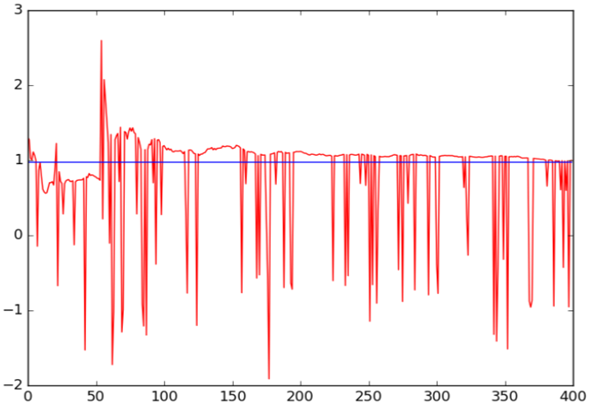
\includegraphics[scale=0.6]{AlgBandit}
	\caption[Resultado de la selección de brazo usando \textit{bandits}]{Selección de la mejor acción usando el algoritmo de los \textit{bandits}}
	\label{AlgBandit}
\end{figure}

La oscilación de la línea roja se produce por la exploración que el algoritmo hace de otras alternativas diferentes a la que en cada momento parece ser la mejor. No se esperan los mismos valores cada vez que se esté probando el mismo \textit{bandit}, porque los valores que recibe son los que fueron distorsionados con el ruido. 

\subsection{Generador de la matriz de adyacencia}

Posteriormente se implementó un código que genera aleatoriamente matrices de adyacencia del grafo por etapas. Estas matrices deben ser escalonadas, deben obedecer a los requisitos de precedencia de nodos entre etapas y deben tener al menos un 1 en cada fila para garantizar la conexión de las etapas. El pseudocódigo \ref{Matriz} corresponde a tales características.

Este algoritmo recibe los datos de número de etapas y número de nodos por cada etapa que ya han de estar definidos con anterioridad.

\begin{algorithm} [h]
\caption{Genera-matriz(L=Cantidad de etapas, M[L]=Nodos por etapa} 
\label{Matriz}
\begin{algorithmic}[1]
\STATE Calculate: n=Cantidad de nodos
\STATE Generate: Ad[nxn] = zeros
\STATE nodoi=0
\STATE nodofin= nodoi+M[0]-1
\FOR{l = 1 \TO L-1}
    \FOR{i in range(nodoi, nodofin+1)}
        \STATE nodohi=nodofin+1
        \STATE nodohfin= nodohi+M[l+1]-1
        \STATE sumafila=0
        \FOR{j in range(nodohi, nodohfin+1)}
            \STATE arg = np.random.randint(2, size=1)
            \STATE A[i,j] = arg 
            \STATE sumafila += A[i,j]
            \IF{umafila == 0}
                \STATE  A[i,j] = 1
            \ENDIF
        \ENDFOR
    \ENDFOR
    \STATE nodoi=nodohi
    \STATE nodofin=nodohfin
\ENDFOR     
\STATE Imprima('A ',A)
\end{algorithmic}
\end{algorithm}

Este código también se probó varias veces y siempre arrojó resultados adecuados de matrices escalonadas, adecuadas para el grafo por etapas diseñado, como el ejemplo que se muestra en la figura \ref{MatrizAy}. 

\begin{figure} [H]
    \label{Resul2}
	\centering
	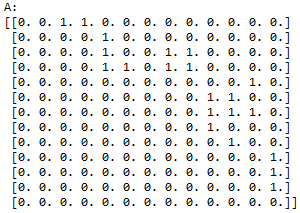
\includegraphics[scale=0.8]{MatrizAy}
	\caption{Resultado de la matriz de adyacencia para un grafo por etapas}
	\label{MatrizAy}
\end{figure}

\subsubsection{Generación de una ruta aleatoria}

Se implementó la fusión del algoritmo para la generación de la matriz de adyacencia, con el que genera los valores asociados a cada nodo o \textit{bandit}; el pseudocódigo correspondiente se probó con valores aleatorios, obteniendo siempre la matriz escalonada que se esperaba y los valores asociados a los \textit{bandits}.

Se le adicionó una funcionalidad para que tomara una ruta factible, teniendo en cuenta la matriz de adyacencia para encontrar los vecinos de cada nodo, la cual se presenta en el algoritmo \ref{Ruta}. Las pruebas que se hicieron funcionaron siempre correctamente.

\begin{algorithm} [h]
\caption{Genera-rutas(L=Cantidad de etapas, A=Matriz de adyacencia} 
\label{Ruta}
\begin{algorithmic}[1]
\STATE n[0]=0
\FOR{l = 1 \TO L}
    \STATE nzv = np.nonzero(A[o, ])
    \STATE nzv = np.reshape(nzv,-1) :vector de nodos adyacentes
    \FOR{i in range(o, len(nzv)}
        \STATE d = np.random.choice(nzv, 1)
        \STATE R[l]=d
    \ENDFOR   
\ENDFOR
\STATE Imprima('Ruta ',R)
\end{algorithmic}
\end{algorithm}

\textit{Los valores que se asignaron aleatoriamente a los \textit{bandits} sirven para calcular una ganancia total por cada ruta que contenga nodos de las $L$ etapas; esta ganancia equivaldría a la \textit{ganancia real} que se obtendría si se supieran los valores de utilidad asociados a cada \textit{bandit}. Así mismo, en cada iteración que ejecute el código, el autómata recibirá una información distorsionada del valor de cada \textit{bandit}, de acuerdo a la distribución Normal que ya se ha explicado; con estos valores el autómata ha de calcular la ganancia que realmente estará recibiendo al final de las $L$ etapas, a la que en adelante se reconocerá como \textit{ganancia distorsionada}. }

El cálculo de la ganancia distorsionada se muestran en los algoritmos siguientes como $Gain_{path}$, la cual va recogiendo en cada etapa la ganancia del nodo seleccionado $Gan_{orig}$, de acuerdo a los valores de utilidad de los \textit{bandit}, que realmente recibe el autómata y que se generan en cada iteración como $Gan_{n}$.

\subsection{Encontrando la ruta óptima}

\textit{Aquí se presentan dos momentos diferentes: Inicialmente aquel donde la escogencia del siguiente nodo de un camino, solo tiene que estar dentro del conjunto de vecinos del nodo actual, pero todos con la misma probabilidad de ser seleccionados; este modelo se reconocerá como Probabilidades Uniformes. Seguidamente se implementa la generación de la matriz de probabilidades de transición de pasar de un nodo a otro, la cual se basa en un fundamento matemático específico que se presentó en la sección \ref{mat}, modelo que se espera que converja a una única respuesta con la mejor ruta encontrada; y este se reconocerá como Probabilidad Modelada.}

\subsection{Búsqueda con probabilidad uniforme}

Inicialmente los nodos de una etapa que sean adyacentes al nodo que ha sido seleccionado en la etapa anterior, tienen una probabilidad uniforme de que sean seleccionados. Este algoritmo se construye básicamente, incluyendo un contador de iteraciones para que el algoritmo de generación de rutas factibles se ejecute una cantidad dada de veces determinada y una selección de la ruta que al final de las iteraciones hubiera obtenido la ganancia promedio, para entregarla como respuesta. 

El pseudocódigo queda como se ve en el cuadro del algoritmo \ref{PsUniforme}, que con los datos de entrada y los generados aleatoriamente para el grafo, calcula una ruta de nodos de cada etapa, solamente teniendo en cuenta que el siguiente nodo forme parte de los vecinos del presente.

\begin{algorithm} [h]
\caption{L-n-bandit-Uniforme(L=Cantidad de etapas, M[L]=Nodos por etapa,
n=Cantidad de nodos)} \label{PsUniforme}
\begin{algorithmic}[1]
\STATE Generate: Ad[nxn] = Matriz de adyacencia
\STATE Generate: B[n] = Bandits reales
\FOR{t = 1 \TO T}
    \STATE Generate: $Gan_{n}$
    \STATE $Gain_{path}$ = 0
    \STATE Initialize: orig = 0
    \STATE Add: orig in path
    \FOR{l = 1 \TO L-1}
        \STATE Generate: $nvz_{orig}$ = vecinos de orig
        \STATE Random: ${dest \in nvz_{orig}}$
        \STATE $orig = dest$
        \STATE Add: orig in path
        \STATE $Gain_{path}$ =+ $Gan_{orig}$
     \ENDFOR
     \STATE Imprima: path
\ENDFOR
\end{algorithmic}
\end{algorithm}

\subsection{Búsqueda con probabilidades aprendidas}
Posteriormente se implementó el cálculo de la matriz de probabilidades de transición con las fórmulas explicadas en la sección \ref{mat} cuyo pseudocódigo se muestra en el cuadro algorítmico \ref{Pseudo}. A diferencia del anterior, la selección del nodo siguiente al presente en cada ruta, no solo va a tener en cuenta la vecindad con este último, sino la probabilidad de transición a cada nodo vecino, consignada en la matriz de probabilidad de transición que aquí se genera y se actualiza, de acuerdo a las ganancias que reciba el camino, en cada iteración, como se explica en seguida.

\begin{algorithm} [h]
\caption{L-n-bandit(L=Cantidad de etapas, M[L]=Nodos por etapa )
} 
\label{Pseudo}
\begin{algorithmic}[1]
\STATE Calculate: n=Cantidad de nodos
\STATE Initialize: v[n] = 0
\STATE Generate: Ad[nxn] = Matriz de adyacencia
\STATE Generate: B[n] = Bandits reales
\FOR{t = 1 \TO T}
     \STATE Initialize: orig = 0
     \STATE Add: orig in path
     \STATE $P(i \to j) = \frac{e^{v_j}}{\sum_k A_{i,k} e^{v_k}},$
     \STATE Generate: $Gan_{n}$
     \STATE $Gain_{path}$ = 0
     \FOR{l = 1 \TO L-1}
        \STATE Generate: $nvz_{orig}$ = vecinos de orig
        \STATE Select: $dest \in nvz_{orig}$  by $P(i \to j)$
        \STATE $orig = dest$
        \STATE Add: orig in path
        \STATE $Gain_{path}$ =+ $Gan_{orig}$
     \ENDFOR
     \IF{$Gain_{path} > 0$}
        \STATE v[n+1] = v[n] + $\delta$ by i $\in$ path
     \ELSE
        \STATE v[n+1] = v[n] - $\delta$ by i $\in$ path   
     \ENDIF   
     \STATE Imprima: path
\ENDFOR
\end{algorithmic}
\end{algorithm}

Para la primera iteración se maneja una probabilidad uniforme y para las demás iteraciones, se calculan las probabilidades de transición entre nodos. En cada iteración se selecciona un nodo de la etapa inicial, se calculan sus vecinos o nodos alcanzables y se selecciona el que mayor probabilidad de transición presente, para guardarlo en la ruta y proceder a hacer la búsqueda de sus vecinos en la siguiente etapa, hasta llegar a la última, usando siempre el mismo criterio de selección.

Una vez se conozca la ganancia o pérdida al final de la iteración, se actualizan los valores de utilidad $v$ de cada nodo de esa ruta, de acuerdo a la fórmula \ref{model3}, este valor se utiliza para calcular las nuevas probabilidades de transición con la fórmula \ref{model2}, que se tendrán en cuenta en la siguiente iteración. Cabe anotar que al final de cada etapa solo se afectan las probabilidades de transición de los nodos involucrados en la ruta seleccionada, pero que al iniciar cada iteración se cuenta con todas las modificaciones que hayan sufrido estas probabilidades en las iteraciones anteriores de esta simulación.

Se recuerda que la selección del siguiente vecino está fuertemente influenciada por las probabilidades de transición, constituyéndose en la explotación de los caminos preferidos, pero siempre deja un porcentaje de posibilidad de escoger cualquier nodo que no sea el de mayor probabilidad de transición asociada, lo que permite resolver el problema de la exploración, propio de la teoría de los \textit{bandits}, que garantiza la búsqueda de mejores soluciones que no se han considerado aún.

Al final de las iteraciones definidas, el simulador debe converger a la mejor ruta que haya estudiado, que puede ser la óptima, como se verá en la siguiente sección.

\section{Pruebas}

\subsection{Grafo para las pruebas}

Aunque el algoritmo se ha diseñado para generar grafos aleatorios, se hace necesario generar uno particular para poder comparar los valores resultantes de las ejecuciones del algoritmo con este. Tal grafo debe ser de un tamaño adecuado para poder calcular todas las posibles rutas desde un nodo inicial hasta uno final con sus respectivas ganancias; además, los nodos deberán tener asociados valores de ganancias, de forma que se pueda establecer claramente cuál es la ruta óptima.

\begin{figure}[h]
  \centering
    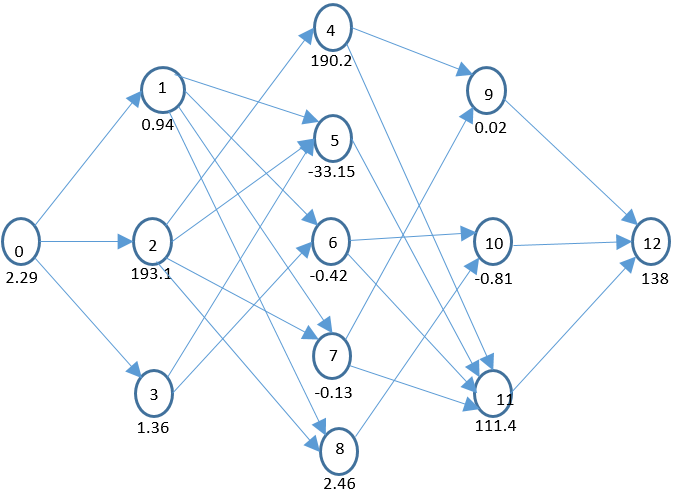
\includegraphics[scale=0.5]{Grafo5L.png}
  \caption[Grafo Modelo]{Grafo Modelo con 5 etapas y 13 nodos}
  \label{Grafomodelo}
\end{figure}

Se realizan estas pruebas entonces, con un grafo de 5 etapas y 13 nodos, dispuestos como se ve en la figura \ref{Grafomodelo}, inicialmente con matriz de adyacencia aleatoria, así como los valores de utilidad de sus \textit{bandits}, pero obligando a que uno de ellos por etapa tenga un mayor valor que los demás, para identificar con facilidad la mejor ruta y así verificar su funcionamiento.


\subsection{Pruebas con probabilidad uniforme}

El algoritmo cuyo pseudocódigo se presentó en el cuadro \ref{PsUniforme}, se ejecutó con 99 intervalos de tiempo. La figura \ref{fig:uniforme} muestra uno de los resultados. 

\begin{figure}[H]
	\centering
	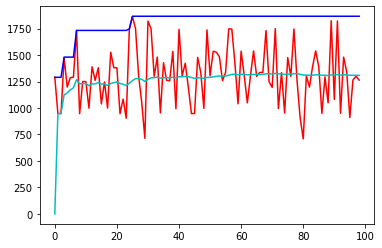
\includegraphics[scale=1]{Uniforme}
	\caption{Resultado con probabilidad uniforme}
	\label{fig:uniforme}
\end{figure}

En esta gráfica, la curva superior azul corresponde a la ganancia real de la mejor ruta probada hasta el momento, calculada con el valor de utilidad asignado a los \textit{bandits}; en la curva roja, la más inestable, se presentan las ganancias distorsionadas obtenidas en cada instante de tiempo por la ruta seleccionada, calculada con los valores distorsionados con ruido para los \textit{bandits}; y en la curva inferior verdosa se muestra el promedio acumulado de estas ganancias, el cual converge a un único valor a través del tiempo, pero no trata de acercarse al valor real.

\subsection{Pruebas con probabilidades aprendidas}

Con 33 iteraciones (T=33) el algoritmo \ref{Pseudo} generó la gráfica de la figura \ref{Resul2}, en la cual se pueden apreciar los valores que van tomado su ganancia y su ganancia promedio, la cual convergió rápidamente hacia el valor de la mejor ganancia real. La mejor ganancia real se calculó para la mejor ruta que el mismo algoritmo haya encontrado: esto permite que el software sea el que estime dicha ruta y su ganancia, sin una intervención manual.

\begin{figure} [H]
	\centering
	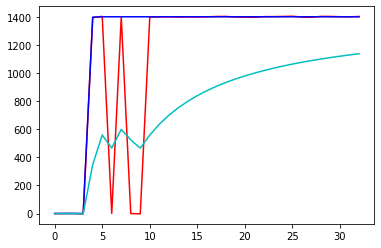
\includegraphics[scale=1]{Resul2}
	\caption{Resultado con probabilidad aprendida}
	\label{Resul2}
\end{figure}
En esta gráfica, al igual que en la del modelo anterior, la curva superior azul corresponde a la ganancia de la mejor ruta probada hasta el momento, calculada con el valor de utilidad real asignado a cada uno de los \textit{bandits}; en la curva más inestable se presentan las ganancias distorcionads obtenidas en cada instante de tiempo por la ruta seleccionada; y en la curva inferior verdosa se muestra el promedio acumulado de estas ganancias, el cual, trata de acercarse a la curva de la ganancia real. 

De otra parte, para estimar el comportamiento del algoritmo se dejan fijos en el grafo los datos de la matriz de adyacencia y del vector de valores de utilidad reales de los \textit{bandits}, para ejecutar los experimentos que se explican en el siguiente capítulo.


%y se estima una ganancia que se genera aleatoriamente a una desviación estándar de su \textit{bandit} ... La decisión de usar una generación de números aleatorios que siguen una distribución normal con media en cero y desviación estándar en 1, es porque es la utilizada en la literatura de aprendizaje por refuerzo \citep{sutton1992reinforcement}, con la cual se ha probado el funcionamiento del modelo de decisión \textit{n-armed bandit}. 